%%%%%%%%%%%%%%%%%%%%%%%%%%%%%%%%%%%%%%%%%%%%%%%%%%%%%%%%%%%%%%%%%%%%%%%%%%%%%%%%
%                              Document Settings                               %
%%%%%%%%%%%%%%%%%%%%%%%%%%%%%%%%%%%%%%%%%%%%%%%%%%%%%%%%%%%%%%%%%%%%%%%%%%%%%%%%

\documentclass[a4paper,12pt]{article}

%%%%%%%%%%%%%%%%%%%%%%%%%%%%%%%%%%%%%%%%%%%%%%%%%%%%%%%%%%%%%%%%%%%%%%%%%%%%%%%%
%                                   Margins                                    %
%%%%%%%%%%%%%%%%%%%%%%%%%%%%%%%%%%%%%%%%%%%%%%%%%%%%%%%%%%%%%%%%%%%%%%%%%%%%%%%%

% The 'geometry' package replaces manual margin adjustments.
% 'a4paper' sets the paper size, and 'margin' sets uniform spacing.
% 'top' and 'bottom' are adjusted here to give more vertical space.
\usepackage[a4paper, top=2.5cm, bottom=2.5cm, left=3cm, right=3cm]{geometry}

%%%%%%%%%%%%%%%%%%%%%%%%%%%%%%%%%%%%%%%%%%%%%%%%%%%%%%%%%%%%%%%%%%%%%%%%%%%%%%%%
%                                   Packages                                   %
%%%%%%%%%%%%%%%%%%%%%%%%%%%%%%%%%%%%%%%%%%%%%%%%%%%%%%%%%%%%%%%%%%%%%%%%%%%%%%%%
%   Equation and Unit Formatting
\usepackage{amsmath}                % Essential for math formulas and symbol
\usepackage{amsfonts}               % Provides additional mathematical fonts
\usepackage{siunitx}                % The gold standard for units and scientific notation (e.g., 10 \degree C)
\usepackage{subcaption}             % Allows side-by-side figures with sub-labels

%   Figure and Table Formatting
\usepackage[pdftex]{graphicx}       % Allows the inclusion of images (PNG, JPG, PDF)
\usepackage{float}                  % Improves placement of 'floats' like images/tables
\usepackage{booktabs}               % For professional, "cleaner" looking tables (rules like \toprule)
\usepackage{array}                  % Provides more flexibility for table column alignment
\graphicspath{/Images}				% Specify a default path for images

%   Referencing, Citations, and Indexing
\usepackage[style=ieee]{biblatex}   % Manages citations and bibliography using IEEE style
\usepackage[hidelinks]{hyperref}    % Adds clickable links to the TOC and citations
\usepackage{cleveref}               % Smarter cross-referencing: automatically writes "Figure 1" or "Table 2"
\usepackage{imakeidx}               % Enables the creation of an index section
\makeindex
\addbibresource{references.bib}		% Specify path for references.bib

%   Inserting Code Blocks
\usepackage{listings}               % Formats and includes raw source code into the doc
\lstset{breaklines = true}			% Makes code wrap around when put into pdf
\usepackage{matlab-prettifier}		% Insert Matlab Code


%   Other Quality of Life Changes   %
\usepackage[T1]{fontenc}            % Handles font encoding for special characters
\usepackage{parskip}                % Replaces paragraph indents with vertical spacing
\usepackage{microtype}              % Subtly improves typography and prevents awkward line breaks
\usepackage{xcolor}                 % Allows for colored text, useful for code or highlighting
\def\thesection{\arabic{section}}	% Sets numbering for sections to arabic numerals
%\usepackage{lettrine}              % Used for dropped capital letters at starts of sections
%\usepackage{fancyhdr}              % Custom headers and footers for that professional "University" look

% For pseudo-code
\usepackage{algorithm}
\usepackage{algpseudocode}
\usepackage{forest}


%%%%%%%%%%%%%%%%%%%%%%%%%%%%%%%%%%%%%%%%%%%%%%%%%%%%%%%%%%%%%%%%%%%%%%%%%%%%%%%%
%                                   Document                                   %
%%%%%%%%%%%%%%%%%%%%%%%%%%%%%%%%%%%%%%%%%%%%%%%%%%%%%%%%%%%%%%%%%%%%%%%%%%%%%%%%

\begin{document}
	
	% Title page
	% Title page
\begin{titlepage}
	\begin{center}
	
		% University Logo
		
\includegraphics[width=0.6\textwidth]{./Images/up_logo_doc.jpg}\\[2.0cm]    
	
		% Department Title
		\textsc{\LARGE EBB 320}\\[1.0cm]
	
		% Module Tile
		\textsc{\Large Control Systems}\\[0.75cm]

		% Assignment Title
		\textsc{Practical 1: Hardware Implementation and System Identification}\\[1.0cm]
		
		% Students/Contributors Table
		\begin{table}[H]
			\centering
			\begin{tabular}{|m{4.25cm}|m{3.5cm}|m{2.5cm}|m{3cm} m{0cm}|}
				\hline
				\multicolumn{1}{|c|}{\textbf{Name and Surname}}		&
				\multicolumn{1}{c|}{\textbf{Student Number}} 		&
				\multicolumn{1}{c|}{\textbf{Signature}} 			& 
				\multicolumn{1}{c}{\textbf{\% Contribution}} 	    & \\
				\hline
				S. Tudent	& 12345678 && \center{20} & \\[0.75cm]
				\hline
				Cornelis Claasen& 24704611 &
\includegraphics[width=2.5cm]{Images/CW Claasen.jpeg}& \center{33} & \\[0.75cm]
				\hline
				B.J. Mncube& 23700816 &
\includegraphics[width=2.5cm]{Images/IMG_9847.jpeg}& \center{33} & \\[0.75cm]
				\hline
			\end{tabular}
		\end{table}
		
	\end{center}

	% Report Declaration		
	\noindent By signing this assignment we confirm that we have read and are aware of the University of Pretoria's policy on academic dishonesty and plagiarism and we declare that the work submitted in this assignment is our own as delimited by the mentioned policies. We explicitly declare that no parts of this assignment have been copied from current or previous students' work or any other sources (including the internet), whether copyrighted or not. We understand that we will be subjected to disciplinary actions should it be found that the work we submit here does not comply with the said policies.\index{Declaration}

	\begin{center}

		% Fill page
		\vfill

		% Date
		{\large \today}
		
	\end{center}
	
\end{titlepage}

	% Table of Contents
	\tableofcontents

	\include{Content/intro}
	\section{Theoretical Background}

The accuracy of the estimated transfer function models was evaluated using the Normalized Root Mean Square Error (NRMSE) fit percentage. This metric quantifies how well the simulated model response matches the measured physical data, and is defined as:

\begin{equation}
    \text{Fit (\%)} = 100 \times \left( 1 - \frac{\lVert y - \hat{y} \rVert}{\lVert y - \bar{y} \rVert} \right)
    \label{eq:nrmse}
\end{equation}

where $y$ is the measured output data, $\hat{y}$ is the simulated model output, $\bar{y}$ is the mean of the measured output data, and $\lVert \cdot \rVert$ denotes the Euclidean norm.
	\section{Software and Hardware Design Implementation}
In order to allow for easier future interaction, a command system was introduced. The MCU receives commands over UART as a string with the format: \texttt{<command>, <value>}. These commands are interpreted by the MCU, changing the appropriate values.

\begin{center}
    \begin{tblr}{colspec={X[c]|X[c]}, width=0.9\linewidth}
        \hline
        Command     &   Value Changed   \\
        \hline 
        0           &   Change P        \\
        1           &   Change I        \\
        2           &   Change D        \\
        3           &   Change Setpoint \\
        4           &   Change Disturbance Value \\
        5           &   Change Duty Cycle  \\
        6           &   Change PWM Output   \\
        7           &   Change Start Flag\\
        \hline
    \end{tblr}
\end{center}

If the start variable is set, then the sampling process begins. First a timer is started, the PWM output flags variable is then checked to see which PWM signals must be set, and finally the samples are taken.

The samples are converted to temperatures using the temperature calibration equation. A running average of 200 samples is used to filer high frequency noise. The timer started at the beginning of the sampling process is then checked to see if the sampling period has passed, and if not, it waits for the remaining time.
The processed samples are again sent over UART as a string with the format:

\texttt{<Temp1>, <Temp2>, <PWM1>, <PWM2>, <Time>, <Message>}


The \texttt{<Message>} paramater is used to signal error data. Currently the only error message implemented is for if the sampling process takes longer than the set sampling period. (Currently $200~\mathrm{Hz}$)

\begin{figure}
    \centering
    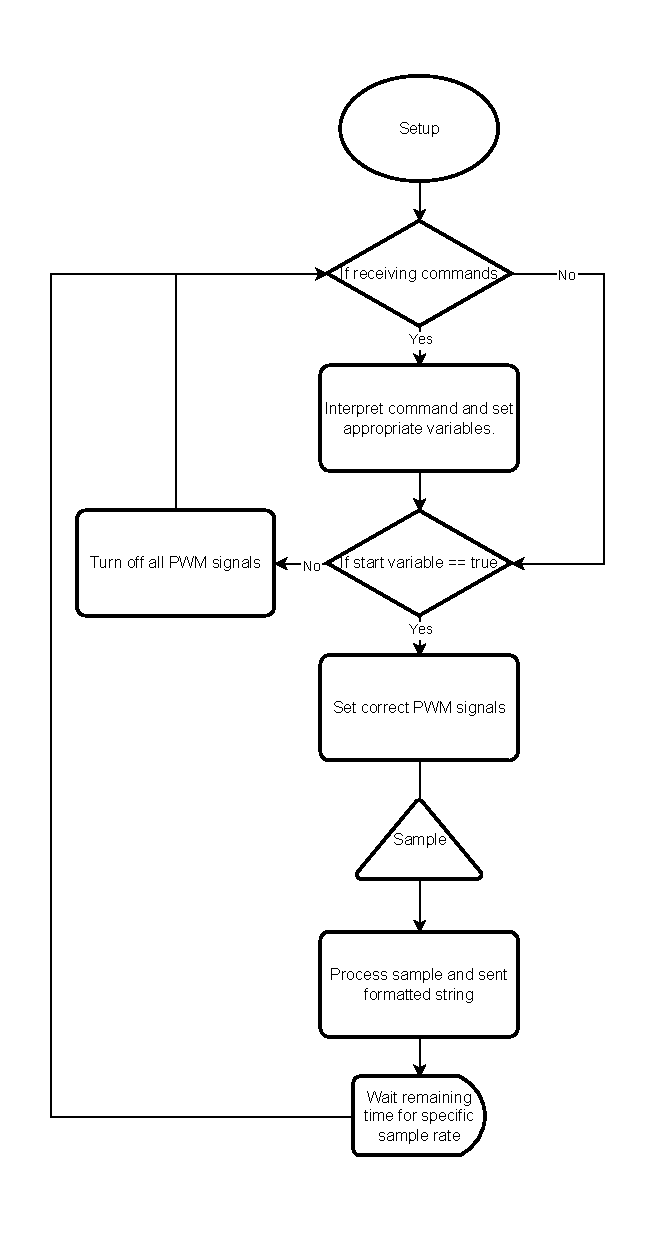
\includegraphics{Images/MCU_Flow1.drawio.pdf}
    \caption{Flow Diagram of MCU Code.}
    \label{fig:MCU_Flow1}
\end{figure}
\pagebreak

\begin{figure}
    \centering
    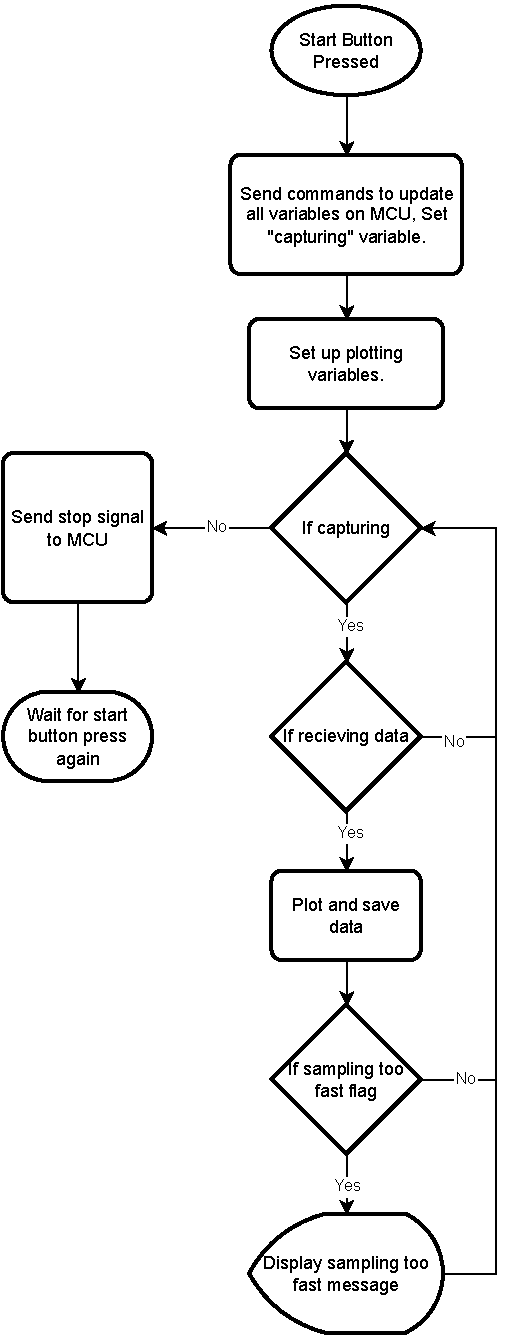
\includegraphics{Images/Matlab_Flow1.drawio.pdf}
    \caption{Flow Diagram of Matlab Code.}
    \label{fig:Matlab_Flow1}
\end{figure}
\pagebreak
	\section{Results}

\subsection{Derived FOPDT transfer functions}
The transfer functions of the system were derived using two different methods, namely the process reaction curve method and transfer function fitting using MATLAB. Each method
yielded a MIMO transfer function matrix with the following mathematical description:

\begin{equation}
    \begin{bmatrix}
        Y_1(s) \\
        Y_2(s)
    \end{bmatrix}
    =
    \begin{bmatrix}
        G_{11}(s) & G_{12}(s) \\
        G_{21}(s) & G_{22}(s)
    \end{bmatrix}
    \begin{bmatrix}
        U_1(s) \\
        U_2(s)
    \end{bmatrix}
\end{equation}

The following table contains these two matrices.

\begin{table}[htbp]
    \centering
    % Increases the vertical space so the fractions don't squash together
    \renewcommand{\arraystretch}{2.5} 
    \caption{Comparison of Transfer Functions: Transfer Function Fitting vs. Process Reaction Curve}
    \label{tab:transfer_function_comparison}
    \begin{tabular}{lcc}
        \hline
        \textbf{Thermal Pathway} & \textbf{Transfer Function Fitting (\texttt{tfest})} & \textbf{Process Reaction Curve} \\
        \hline
        
        % Row 1: G11 (PWM1 to T1)
        $G_{11}(s)$ (PWM 1 $\rightarrow$ T1) & 
        $\frac{-0.1974s + 0.05300}{s^2 + 0.4582s + 0.0034}$ & 
        $\frac{K_{11}}{\tau_{11} s + 1} e^{-\theta_{11} s}$ \\
        
        % Row 2: G12 (PWM2 to T1)
        $G_{12}(s)$ (PWM 2 $\rightarrow$ T1) & 
        $\frac{-0.0156 s + 0.0010}{s^2 + 0.0300 s + 0.0002}$ & 
        $\frac{K_{12}}{\tau_{12} s + 1} e^{-\theta_{12} s}$ \\
        
        % Row 3: G21 (PWM1 to T2)
        $G_{21}(s)$ (PWM 1 $\rightarrow$ T2) & 
        $\frac{-0.0097 s + 0.0016}{s^2 + 0.0268 s + 0.0002}$ & 
        $\frac{K_{21}}{\tau_{21} s + 1} e^{-\theta_{21} s}$ \\
        
        % Row 4: G22 (PWM2 to T2)
        $G_{22}(s)$ (PWM 2 $\rightarrow$ T2) & 
        $\frac{-0.0346 s + 0.0234}{s^2 + 0.3998 s + 0.0024}$ & 
        $\frac{K_{22}}{\tau_{22} s + 1} e^{-\theta_{22} s}$ \\
        
        \hline
    \end{tabular}
\end{table}


\textbf{Comment on the table}

\subsection{Matlab fitting}
The \textbf{tfest} function was used in Matlab to fit the data to a transfer function. The following steps were followed to achieve this:
\\
\\
\textbf{Data Preparation:}
\\
The recorded data was sliced to include a sufficient amount of zero inputs, this is required by the tfest function to properly fit the model. After which the data was broken into a voltage vector (the PWM input), and two temperature vectors 
(temperatures of each of the transistors). The ambient temperature was subtracted from  the temperature vectors and the data was packaged into an iddata object.
\\
\\
\textbf{Model Fitting:}
\\
Three parameters were passed to the tfest function, namely: the iddata object, the number of poles the system has, and the number of zeros the system has.
The number of poles a system has is determined by the number of energy storing elements, in the case of this system the transistors are storing energy in the form
of heat, thus the system has two poles. It is common practise to take the number of zeros of an unknown system as: Zeros $=$ Poles $- 1$. 
The fitted models were then plotted using the compare function as can be seen in the Figure \ref{fig:pwm1_comparison} and Figure \ref{pwm2_comparison} below.



\begin{figure}[htbp]
    \centering
    
\includegraphics[width=1\textwidth]{Images/PWM1Step_Compare.pdf} 
    \caption{Comparison of the physical sensor data against the simulated SIMO transfer function model for PWM 1.}
    \label{fig:pwm1_comparison}
\end{figure}

Figure \ref{fig:pwm1_comparison} displays the fitted model for both $G_{11}$ (top) and $G_{21}$ (bottom) which are similarly accurate; 94.1\% and 94.4\%, on top
of the measured physical data.

\begin{figure}[htbp]
    \centering
    
\includegraphics[width=1\textwidth]{Images/PWM2Step_Compare.pdf} 
    \caption{Comparison of the physical sensor data against the simulated SIMO transfer function model for PWM 2.}
    \label{fig:pwm2_comparison}
\end{figure}



\begin{figure}[htbp]
    \centering
    
\includegraphics[width=1\textwidth]{Images/PWM1Step_TestData.pdf} 
    \caption{Comparison of the physical sensor data for a 50\% duty cycle test case against the simulated SIMO transfer function model for PWM 1.}
    \label{fig:pwm1_test}
\end{figure}

\begin{figure}[htbp]
    \centering
    
\includegraphics[width=1\textwidth]{Images/PWM2Step_TestData.pdf} 
    \caption{Comparison of the physical sensor data for a 50\% duty cycle test case against the simulated SIMO transfer function model for PWM 2.}
    \label{fig:pwm2_test}
\end{figure}
	\section{Discussion}
\subsection{Derived FOPDT transfer functions.}
\subsubsection{Matlab fitting}
The \textbf{tfest} function was used in Matlab to fit the data to a transfer function. The following steps were followed to achieve this:
\\
\\
\textbf{Data Preparation:}
\\
The recorded data was sliced to include a sufficient amount of zero inputs, this is required by the tfest function to properly fit the model. After which the data was broken into a voltage vector (the PWM input), and two temperature vectors 
(temperatures of each of the transistors). The ambient temperature was subtracted from  the temperature vectors and the data was packaged into an iddata object.
\\
\\
\textbf{Model Fitting:}
\\
Three parameters were passed to the tfest function, namely: the iddata object, the number of poles the system has, and the number of zeros the system has.
The number of poles a system has is determined by the number of energy storing elements, in the case of this system the transistors are storing energy in the form
of heat, thus the system has two poles. It is common practise to take the number of zeros of an unknown system as: Zeros $=$ Poles $- 1$.



	\include{Content/conclusion}

	\printbibliography
	\section{Code}

\subsection{Matlab Code}
\lstinputlisting[style=Matlab-editor, caption={App Code For Sampling}]{../Matlab_Code/EBBPrac.m}

\subsection{Model Fit Code}
\lstinputlisting[style=Matlab-editor, caption={Model fitting and plotting code}]{../Matlab_Code/tfest/tfest_code.m}


\subsection{MCU Code}
\lstinputlisting[language=C++]{../MCU_Code/EBB320_Prac1/src/main.cpp}



	% Appendix for tables and figures, might not always be necessary
	\begin{appendix}
		\listoftables
		\listoffigures
	\end{appendix}

\end{document}
